%-----------------------------------------------------------------------------%
\chapter{\babEmpat}
%-----------------------------------------------------------------------------%

\section{Desain Sistem}

Bagian ini menjelaskan tentang desain sistem yang dilakukan sesuai dengan spesifikasi sistem yang telah diajukan. Desain ini dibuat di perangkat lunak GNURadio.

\begin{figure}
	\centering
	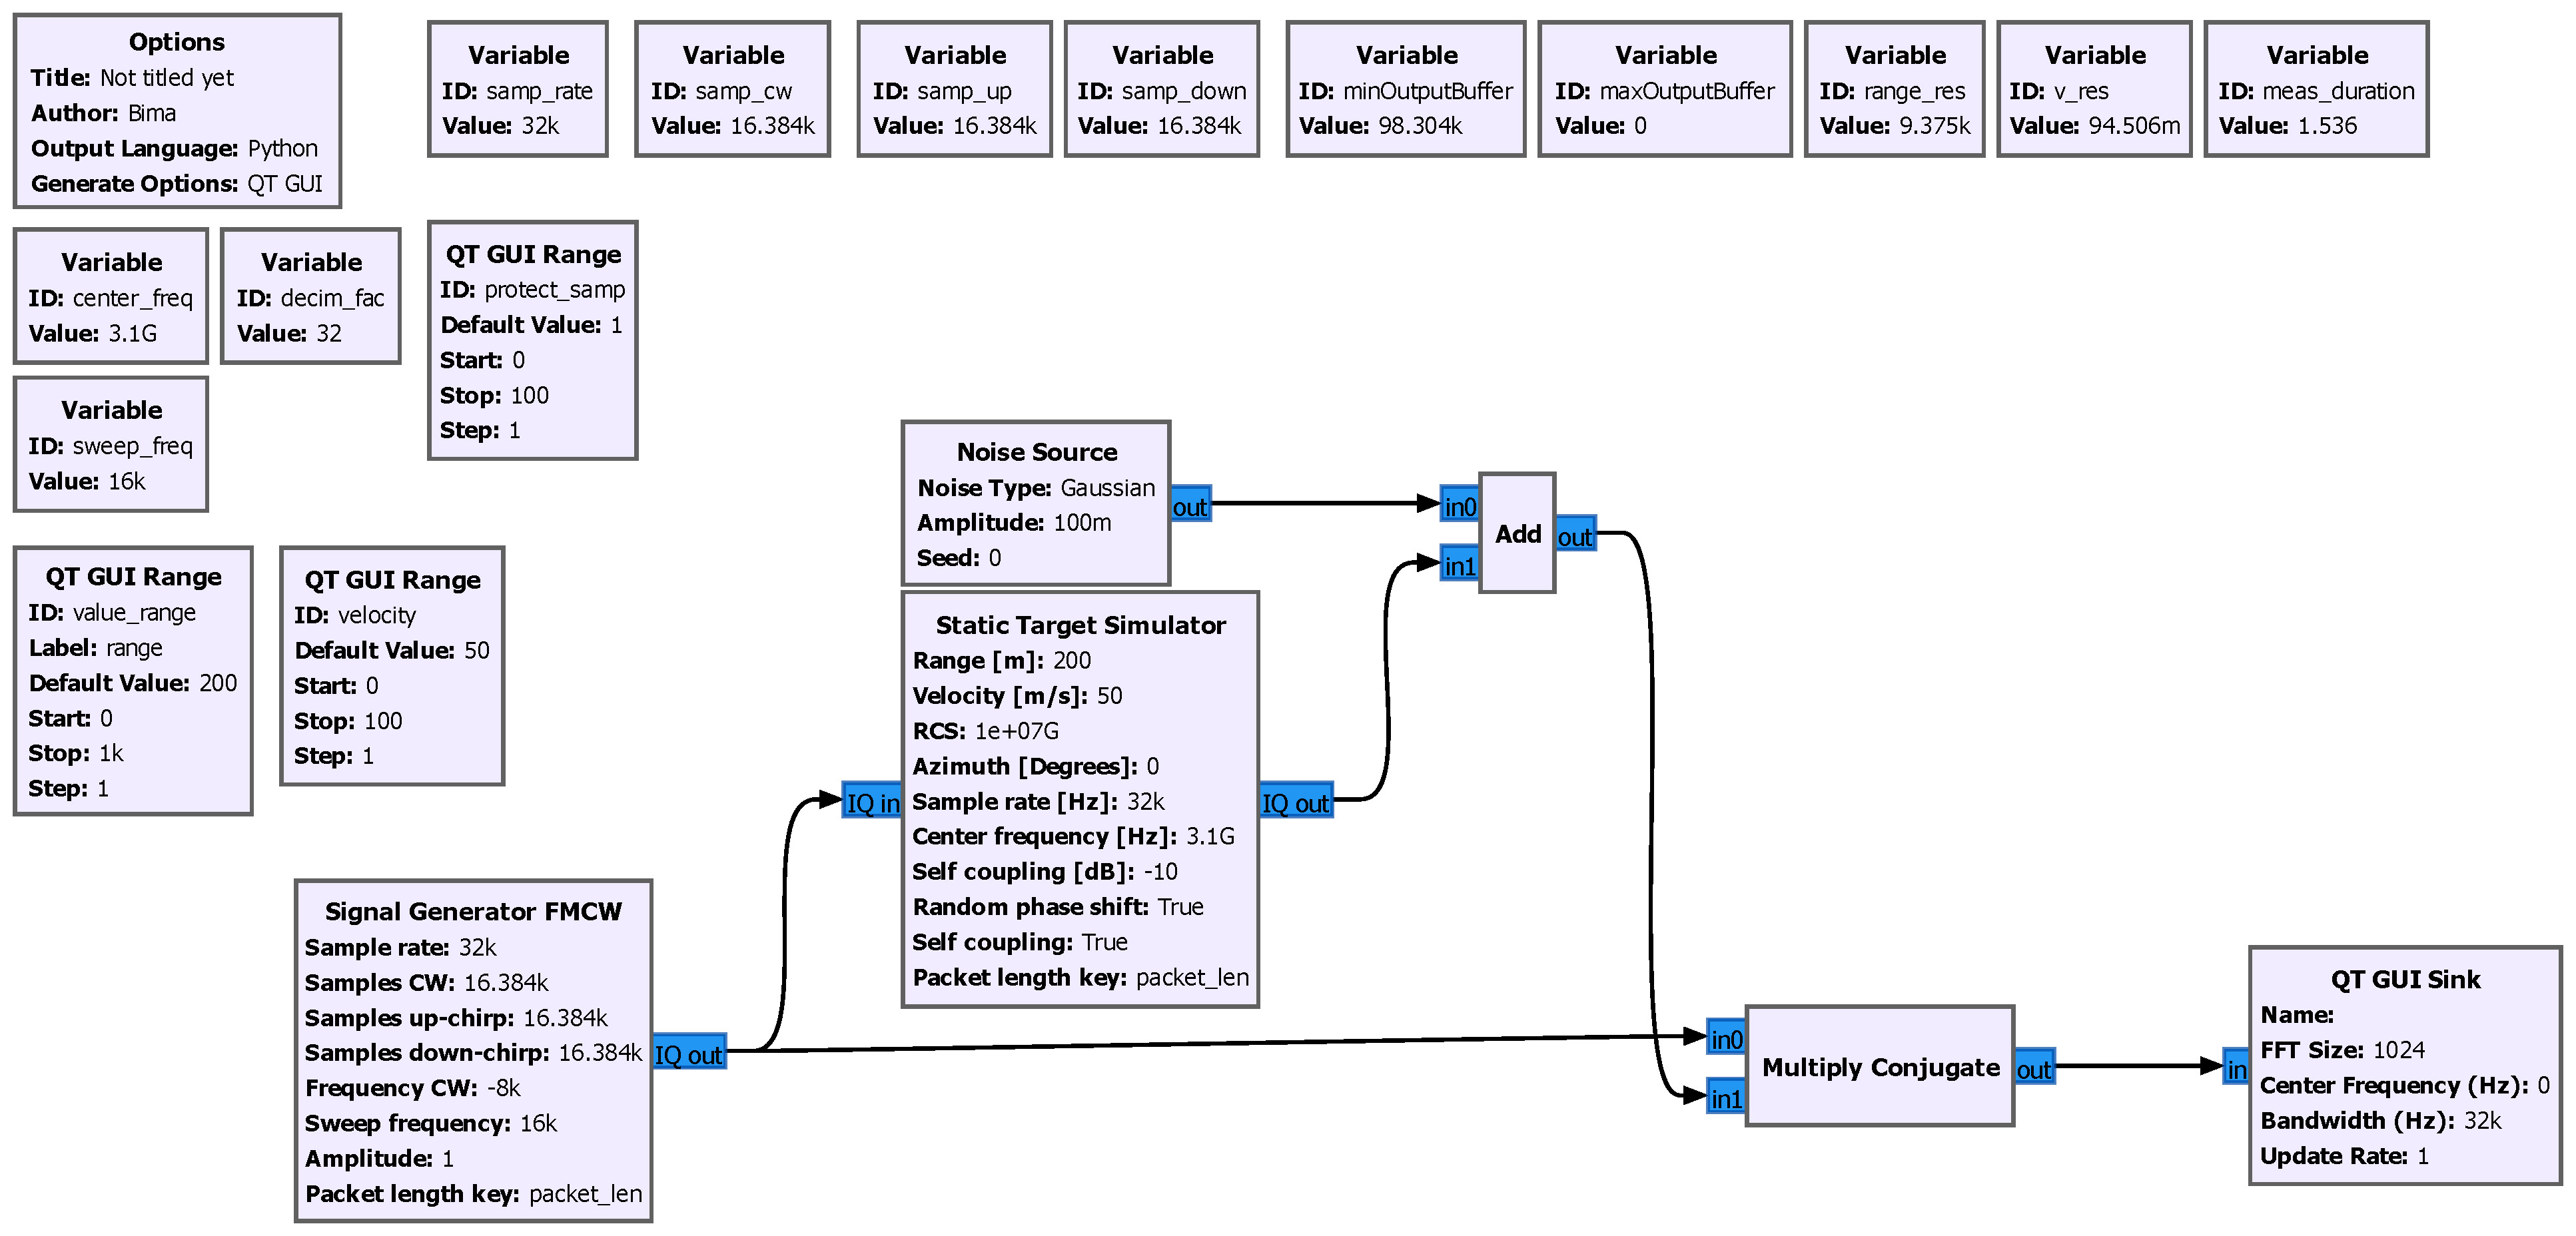
\includegraphics[scale=0.25]{pics/bab4/Simulasi.jpg}
	\caption{Desain Sistem Pada GNURadio}
	\label{fig:DesainSistem}
\end{figure}

Gambar~\ref{fig:DesainSistem} menunjukkan sistem pada GNURadio bila kalkulasi jarak dilakukan secara \textit{real-time}. Namun pada kenyataannya, saat pengukuran dilakukan, terjadi banyak sekali kegagalan, mulai dari \textit{error overflow} dan \textit{underflow}, \textit{error} pada pembacaan nilai jarak yang dihasilkan, hingga kalibrasi sinkronisasi perangkat yang perlu dilakukan tiap sistem diaktifkan.

Sehingga diputuskan bahwa pengambilan hasil dilakukan secara tidak \textit{real-time}, sehingga skema dari sistem yang digunakan di GNURadio berubah. Dalam pengambilan data tidak langsung, juga terjadi \textit{error overflow}, namun hal ini bisa dilewati dengan memanfaatkan kemampuan sistem operasi Linux untuk \textit{mount} dan menyimpan langsung di RAM.

%-----------------------------------------------------------------------------%
\section{Pengukuran Antena}
%-----------------------------------------------------------------------------%
Antena merupakan salah satu faktor penting dalam sistem radar, parameter seperti pola radiasi dan \textit{return loss} merupakan hal yang perlu dipertimbangkan dalam memilih antena. Pada penelitian ini, digunakan antena \textit{log periodic} dengan \textit{bandwidth} yang lebar. Antena identik digunakan sebagai \textit{transmitter} dan \textit{receiver}. Pola radiasi yang didapat pada pengujian antena adalah seperti gambar~\ref{fig:polaRadiasi}.

\begin{figure}
	\centering
	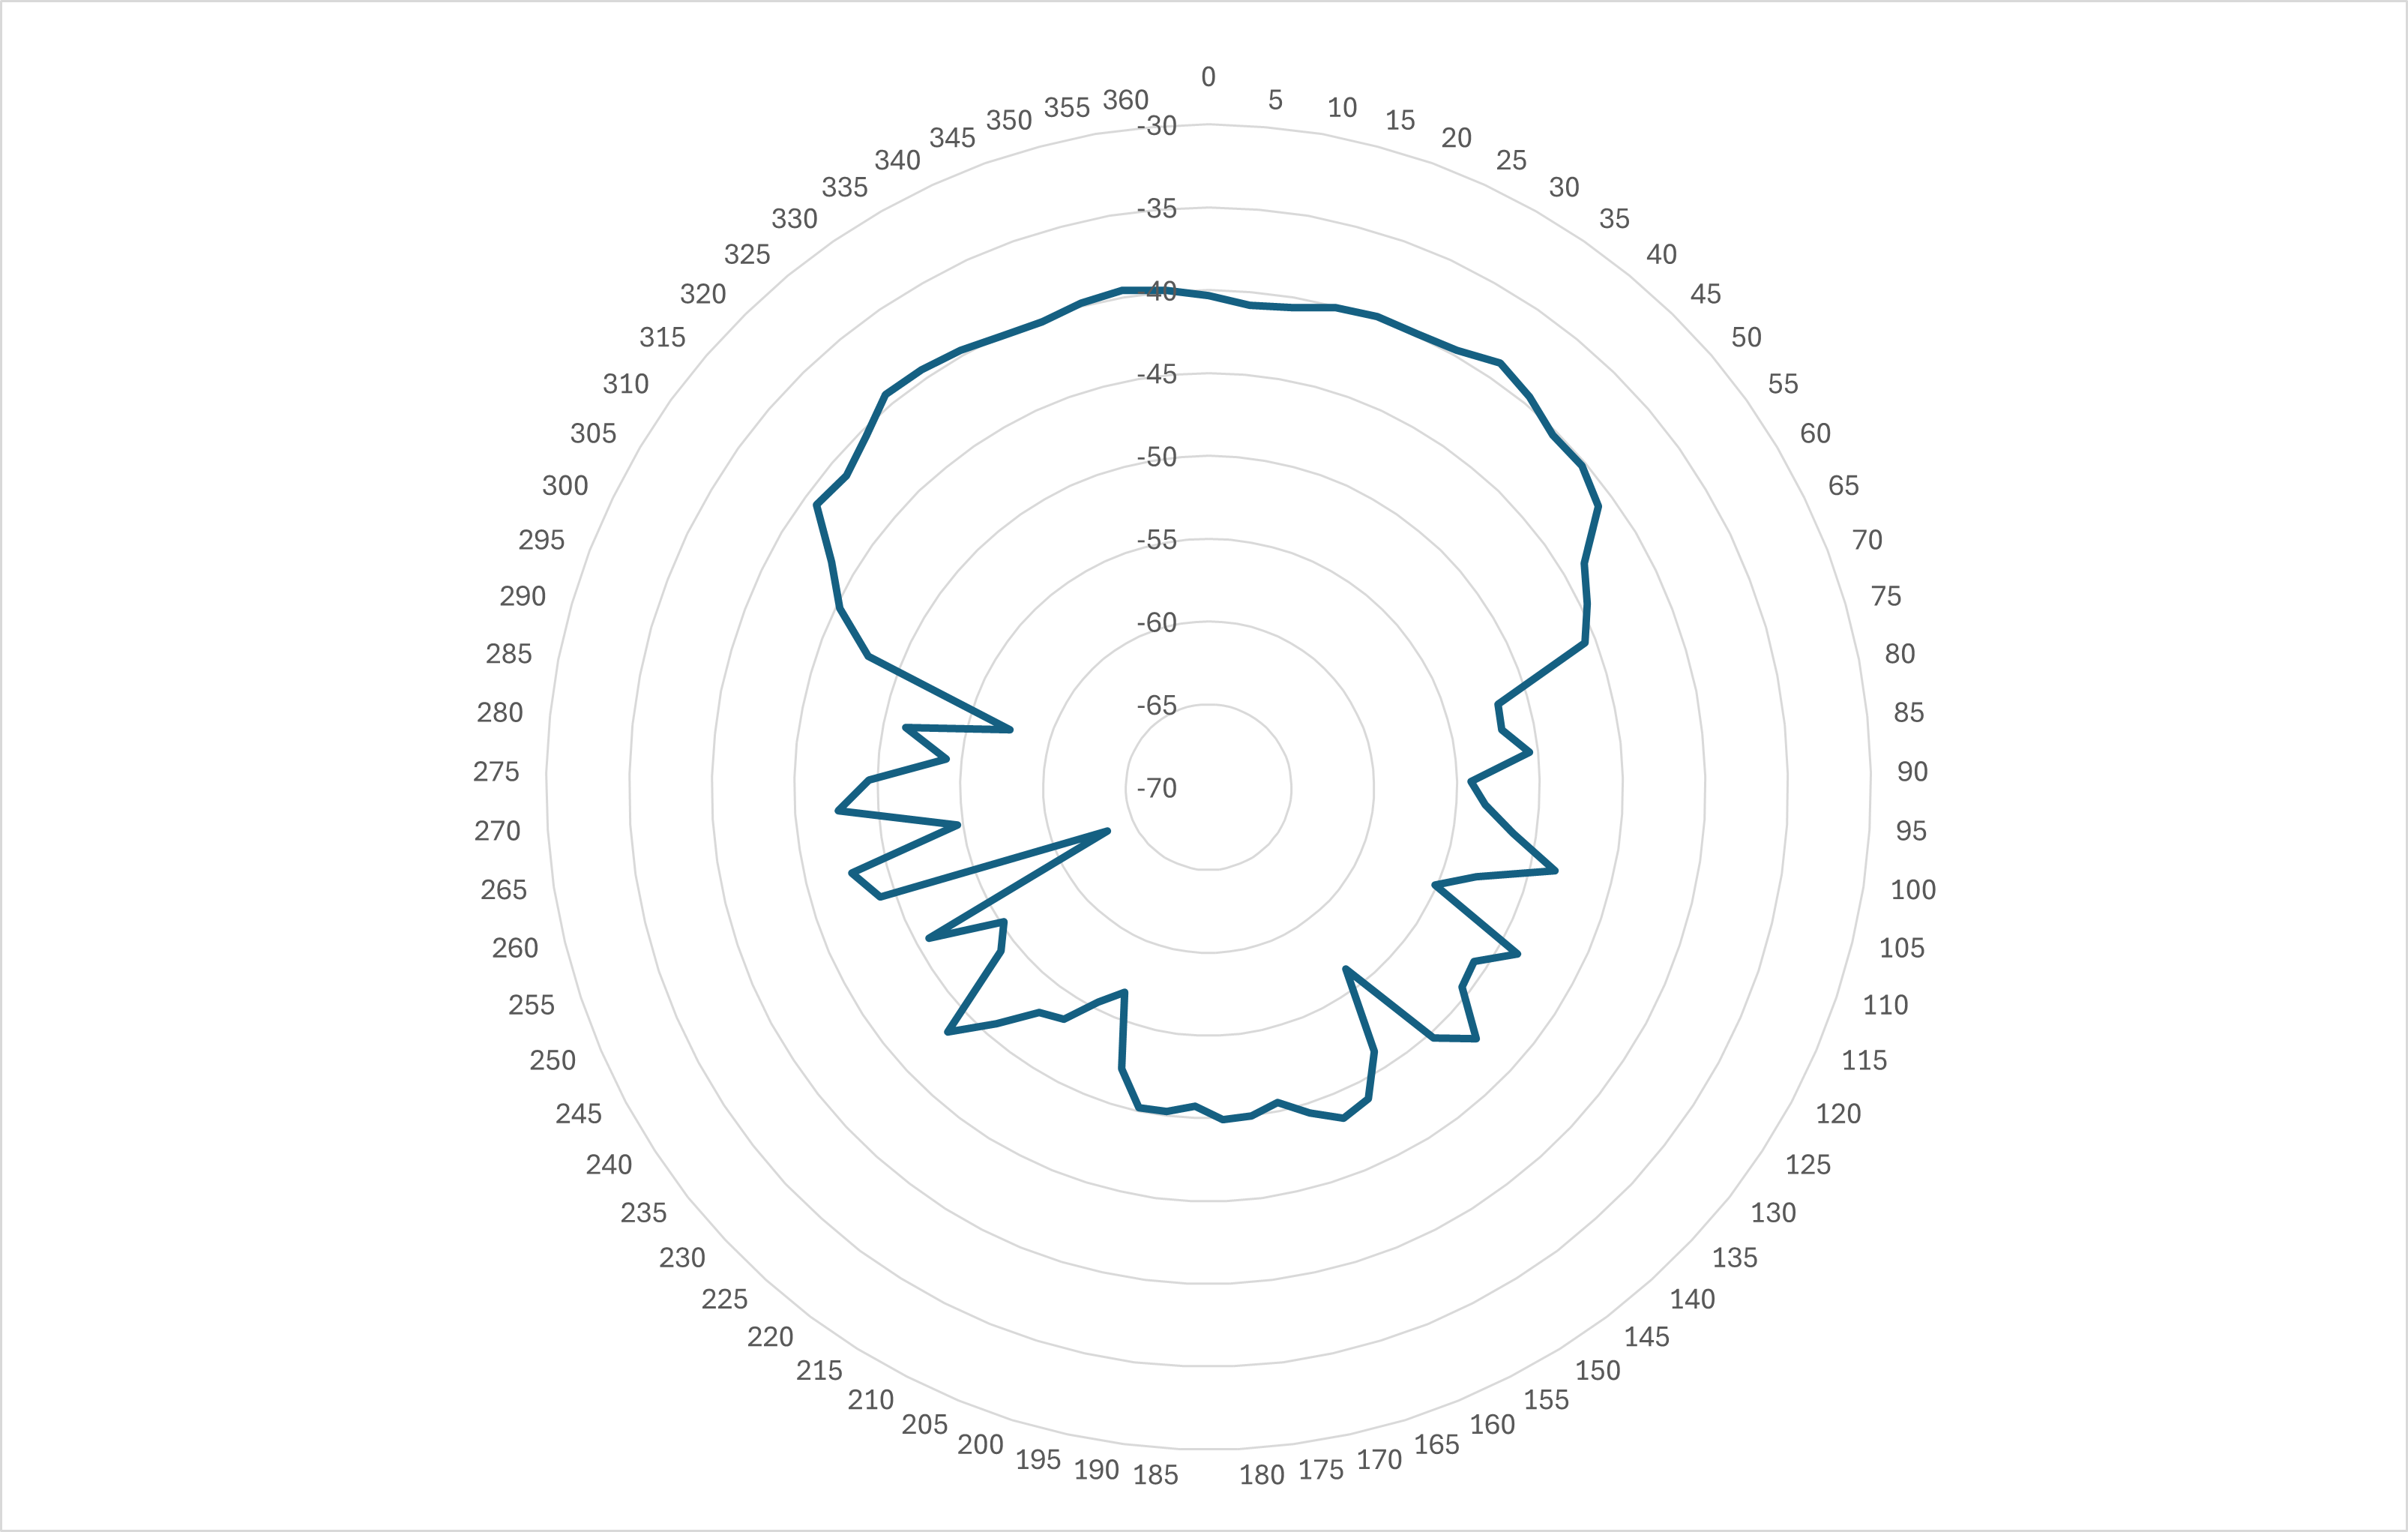
\includegraphics[scale=0.5]{pics/bab4/Ukur Pola Antena 23 Juli/S21A1.png}
	\caption{Hasil pengukuran pola radiasi antena}
	\label{fig:polaRadiasi}
\end{figure}

Gambar~\ref{fig:polaRadiasi} menunjukkan pola radiasi yang bagus untuk digunakan dalam implementasi radar, hal ini ditunjukkan dengan jenis pola radiasi \textit{directional} ke derajat 0. Selain itu, nilai gain dari antena yang digunakan adalah 6 dBi sesuai dengan datasheet yang ada dari antena.

%-----------------------------------------------------------------------------%
\section{Pengambilan Data Jarak}
%-----------------------------------------------------------------------------%

Pengambilan data jarak dilakukan di lapangan upacara Universitas Telkom Surabaya dengan menggunakan kendaraan roda dua. Dengan menggunakan pita ukur dan mengatur jarak kendaraan sesuai dengan parameter pengukuran, pengambilan data jarak dapat dilakukan dengan lancar. Terdapat 3 variasi jarak yang dilakukan, masing masing diulang sebanyak 3 kali untuk menjadi validasi.

\subsection{Jarak 3 Meter}

Pengambilan data jarak 3 meter yang dihitung dari ujung antena hingga ke kendaraan roda dua telah dilakukan seperti pada gambar~\ref{fig:pengambilan3Meter}. Untuk memastikan isolasi antara antena \textit{transmitter} dan antena \textit{receiver}, maka digunakanlah plat yang terbuat dari logam.

\begin{figure}
	\centering
	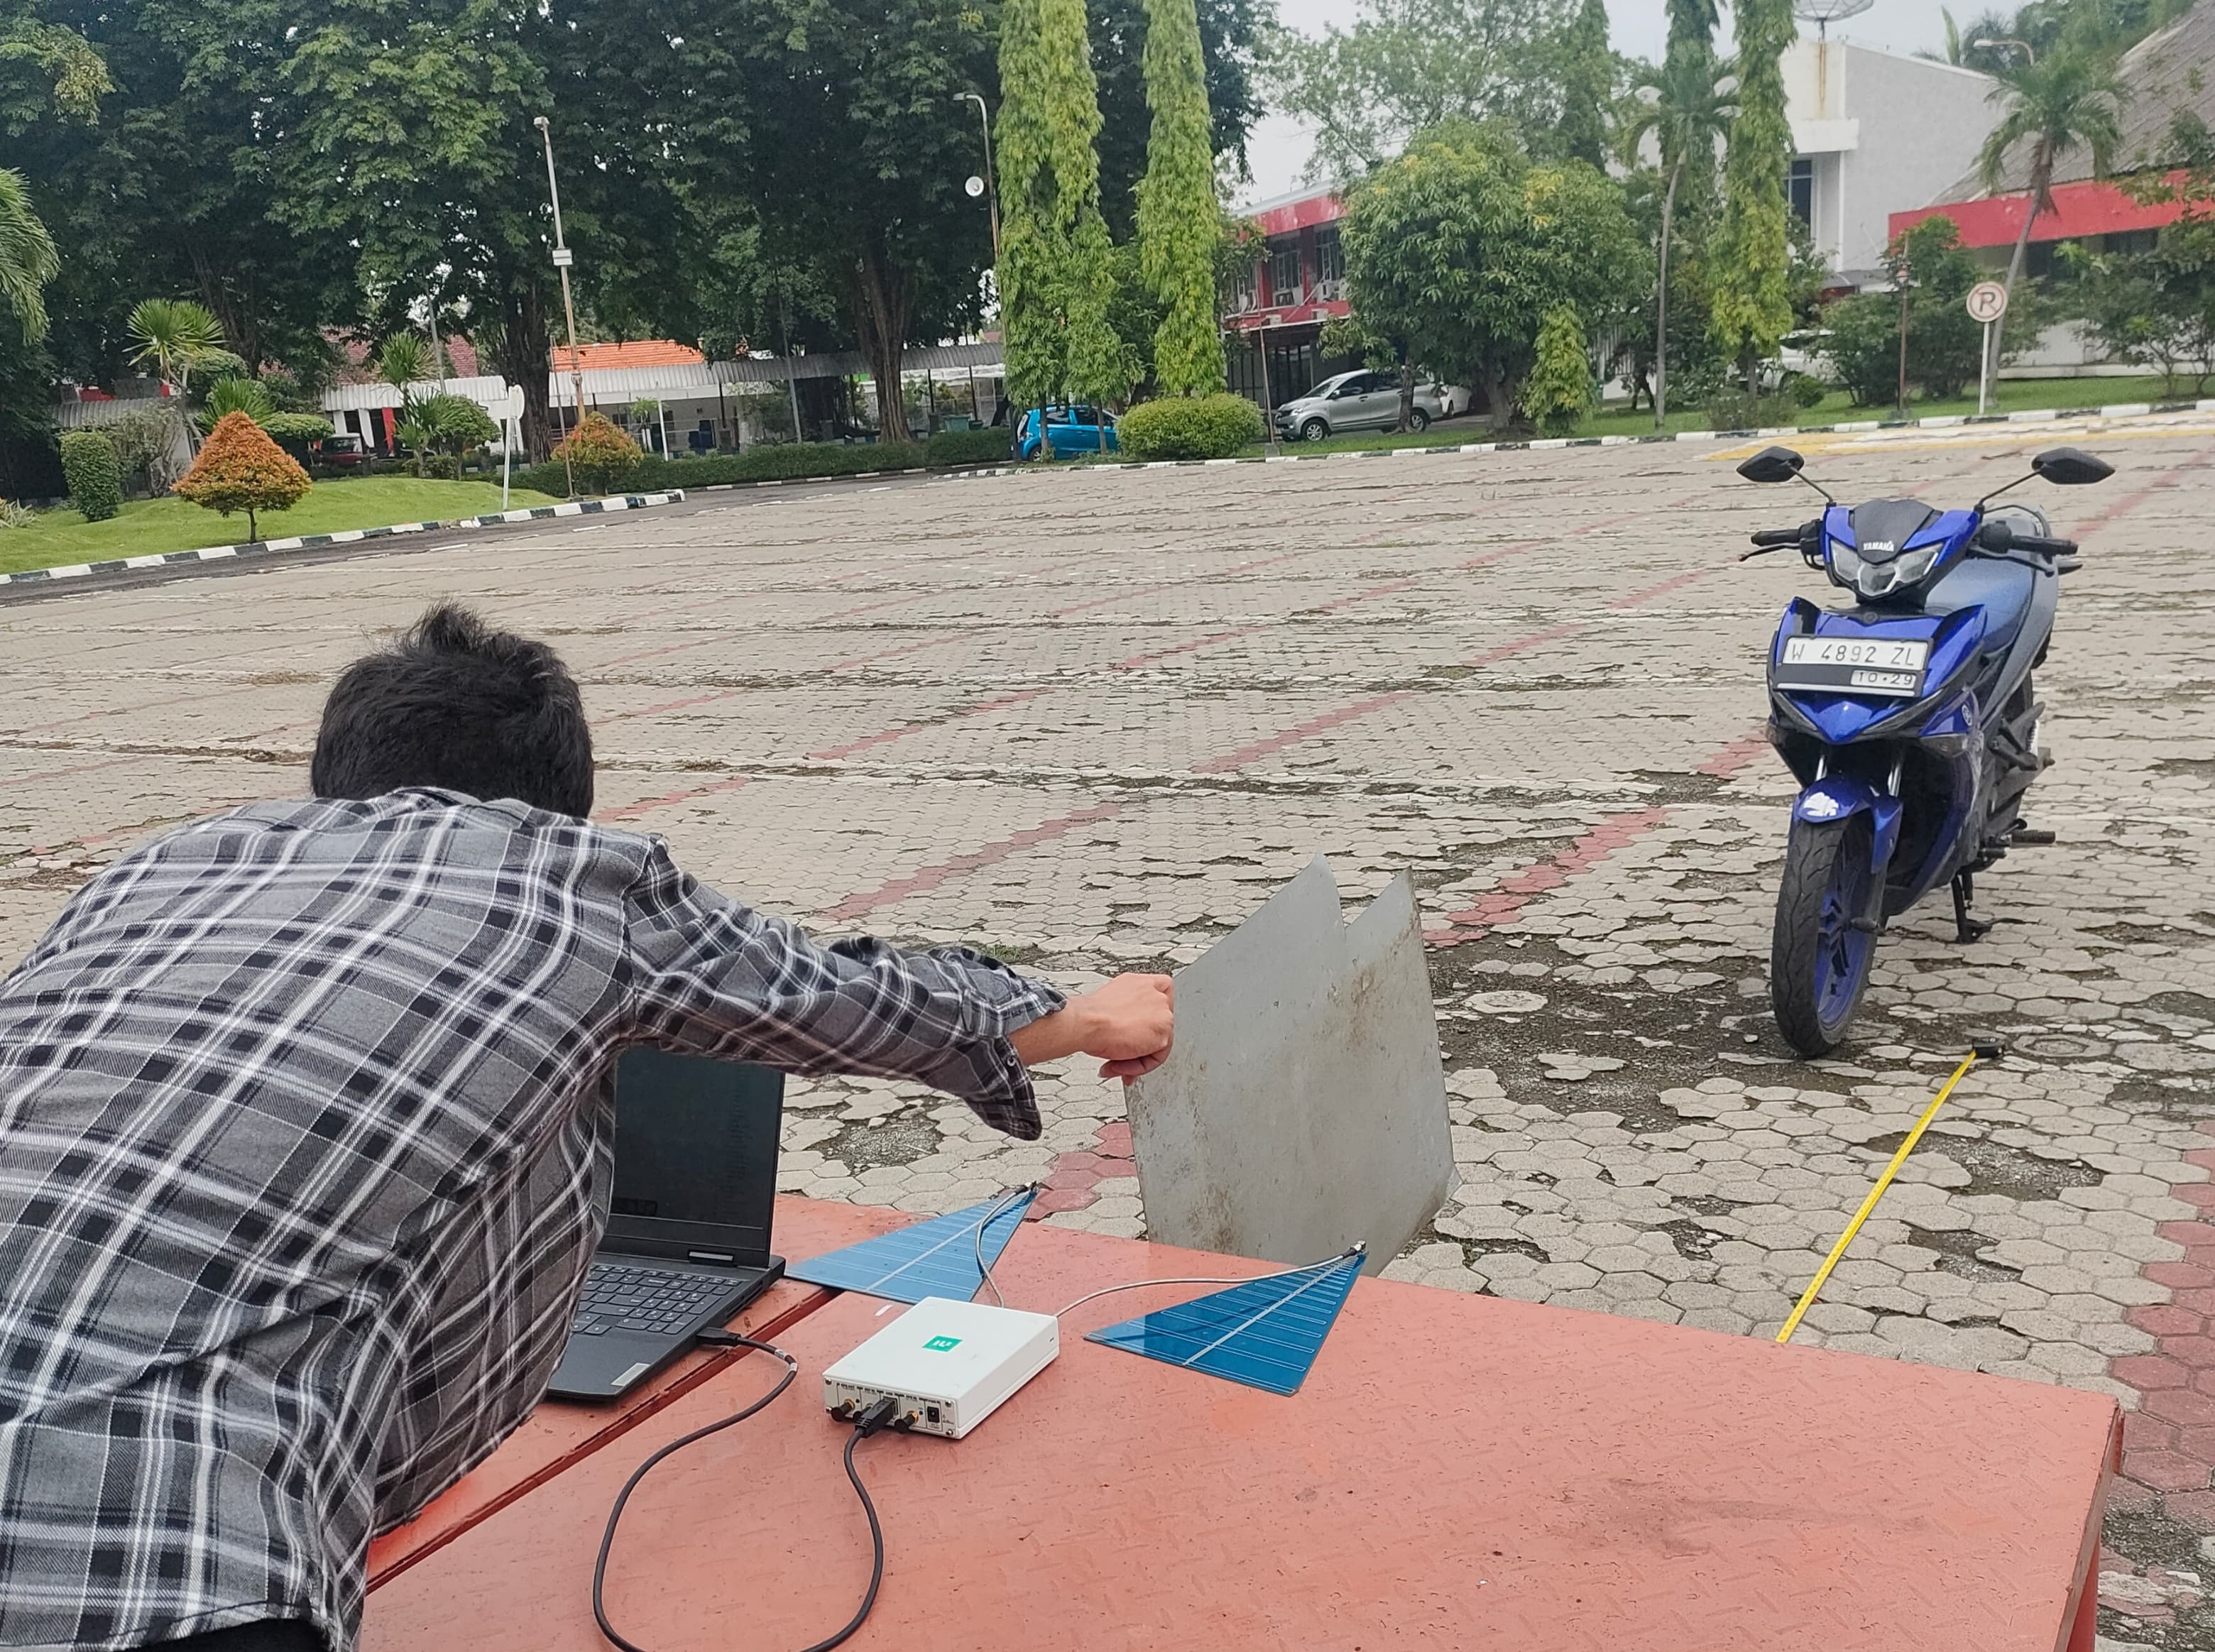
\includegraphics[scale=0.1]{pics/bab4/PengujianRange/3/Masuk.jpg}
	\caption{Pengambilan data jarak 3 meter}
	\label{fig:pengambilan3Meter}
\end{figure}

\subsection{Jarak 6 Meter}

Pengambilan data jarak 6 meter yang juga dilakukan dilokasi yang sama telah dilakukan. Dengan skema perhitungan jarak yang sama dengan pengambilan data jarak 3 meter. Namun pada jarak ini kesulitan dalam mengukur jarak dari ujung antena ditemui karena batas pita ukur yang hanya 3 meter, maka dari itu, pengukuran jarak dilakukan dimulai dari titik sebelumnya yaitu 3 meter.

\begin{figure}
	\centering
	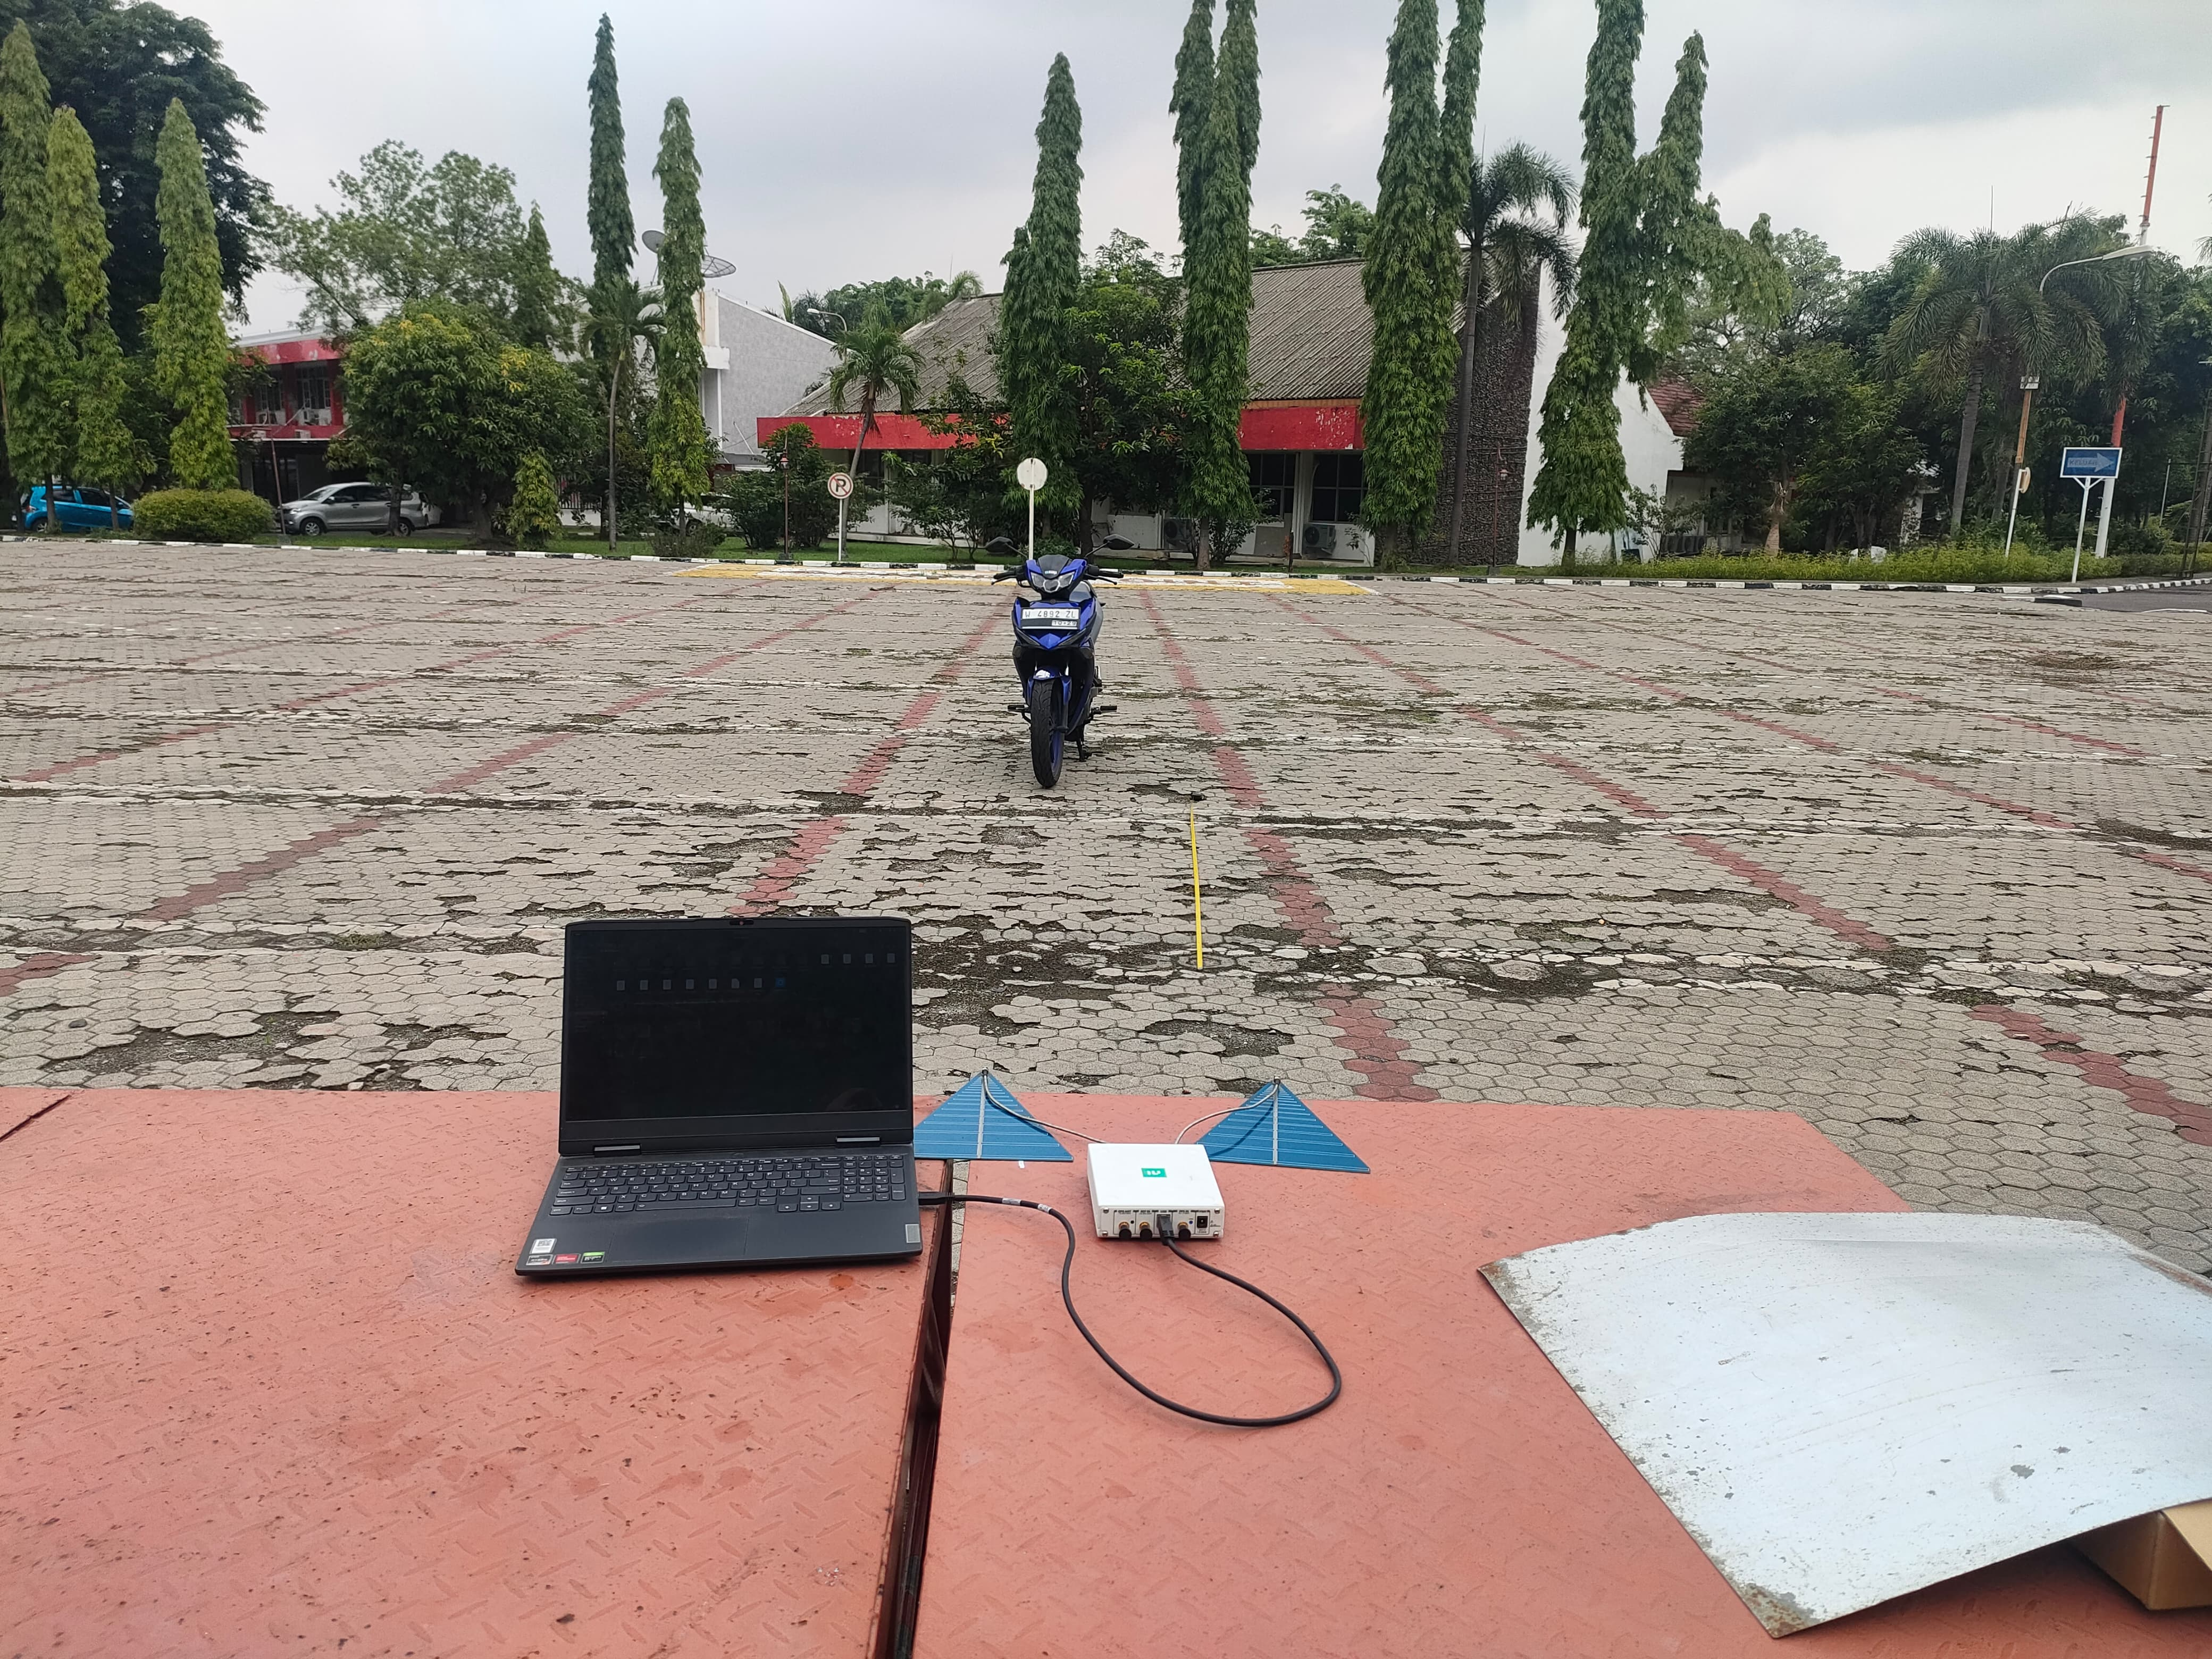
\includegraphics[scale=0.07]{pics/bab4/PengujianRange/6/Masuk.jpg}
	\caption{Pengambilan data jarak 6 meter}
	\label{fig:pengambilan6Meter}
\end{figure}

\subsection{Jarak 9 Meter}

Pengambilan data jarak 9 meter dari ujung antena telah dilaksanakan dengan lancar. Skema pengambilan data jarak sama dengan pengambilan data pada jarak 6 meter. Yaitu dengan memulai perhitungan titik mulai ukur dari titik jarak 6 meter dari antena.

\begin{figure}
	\centering
	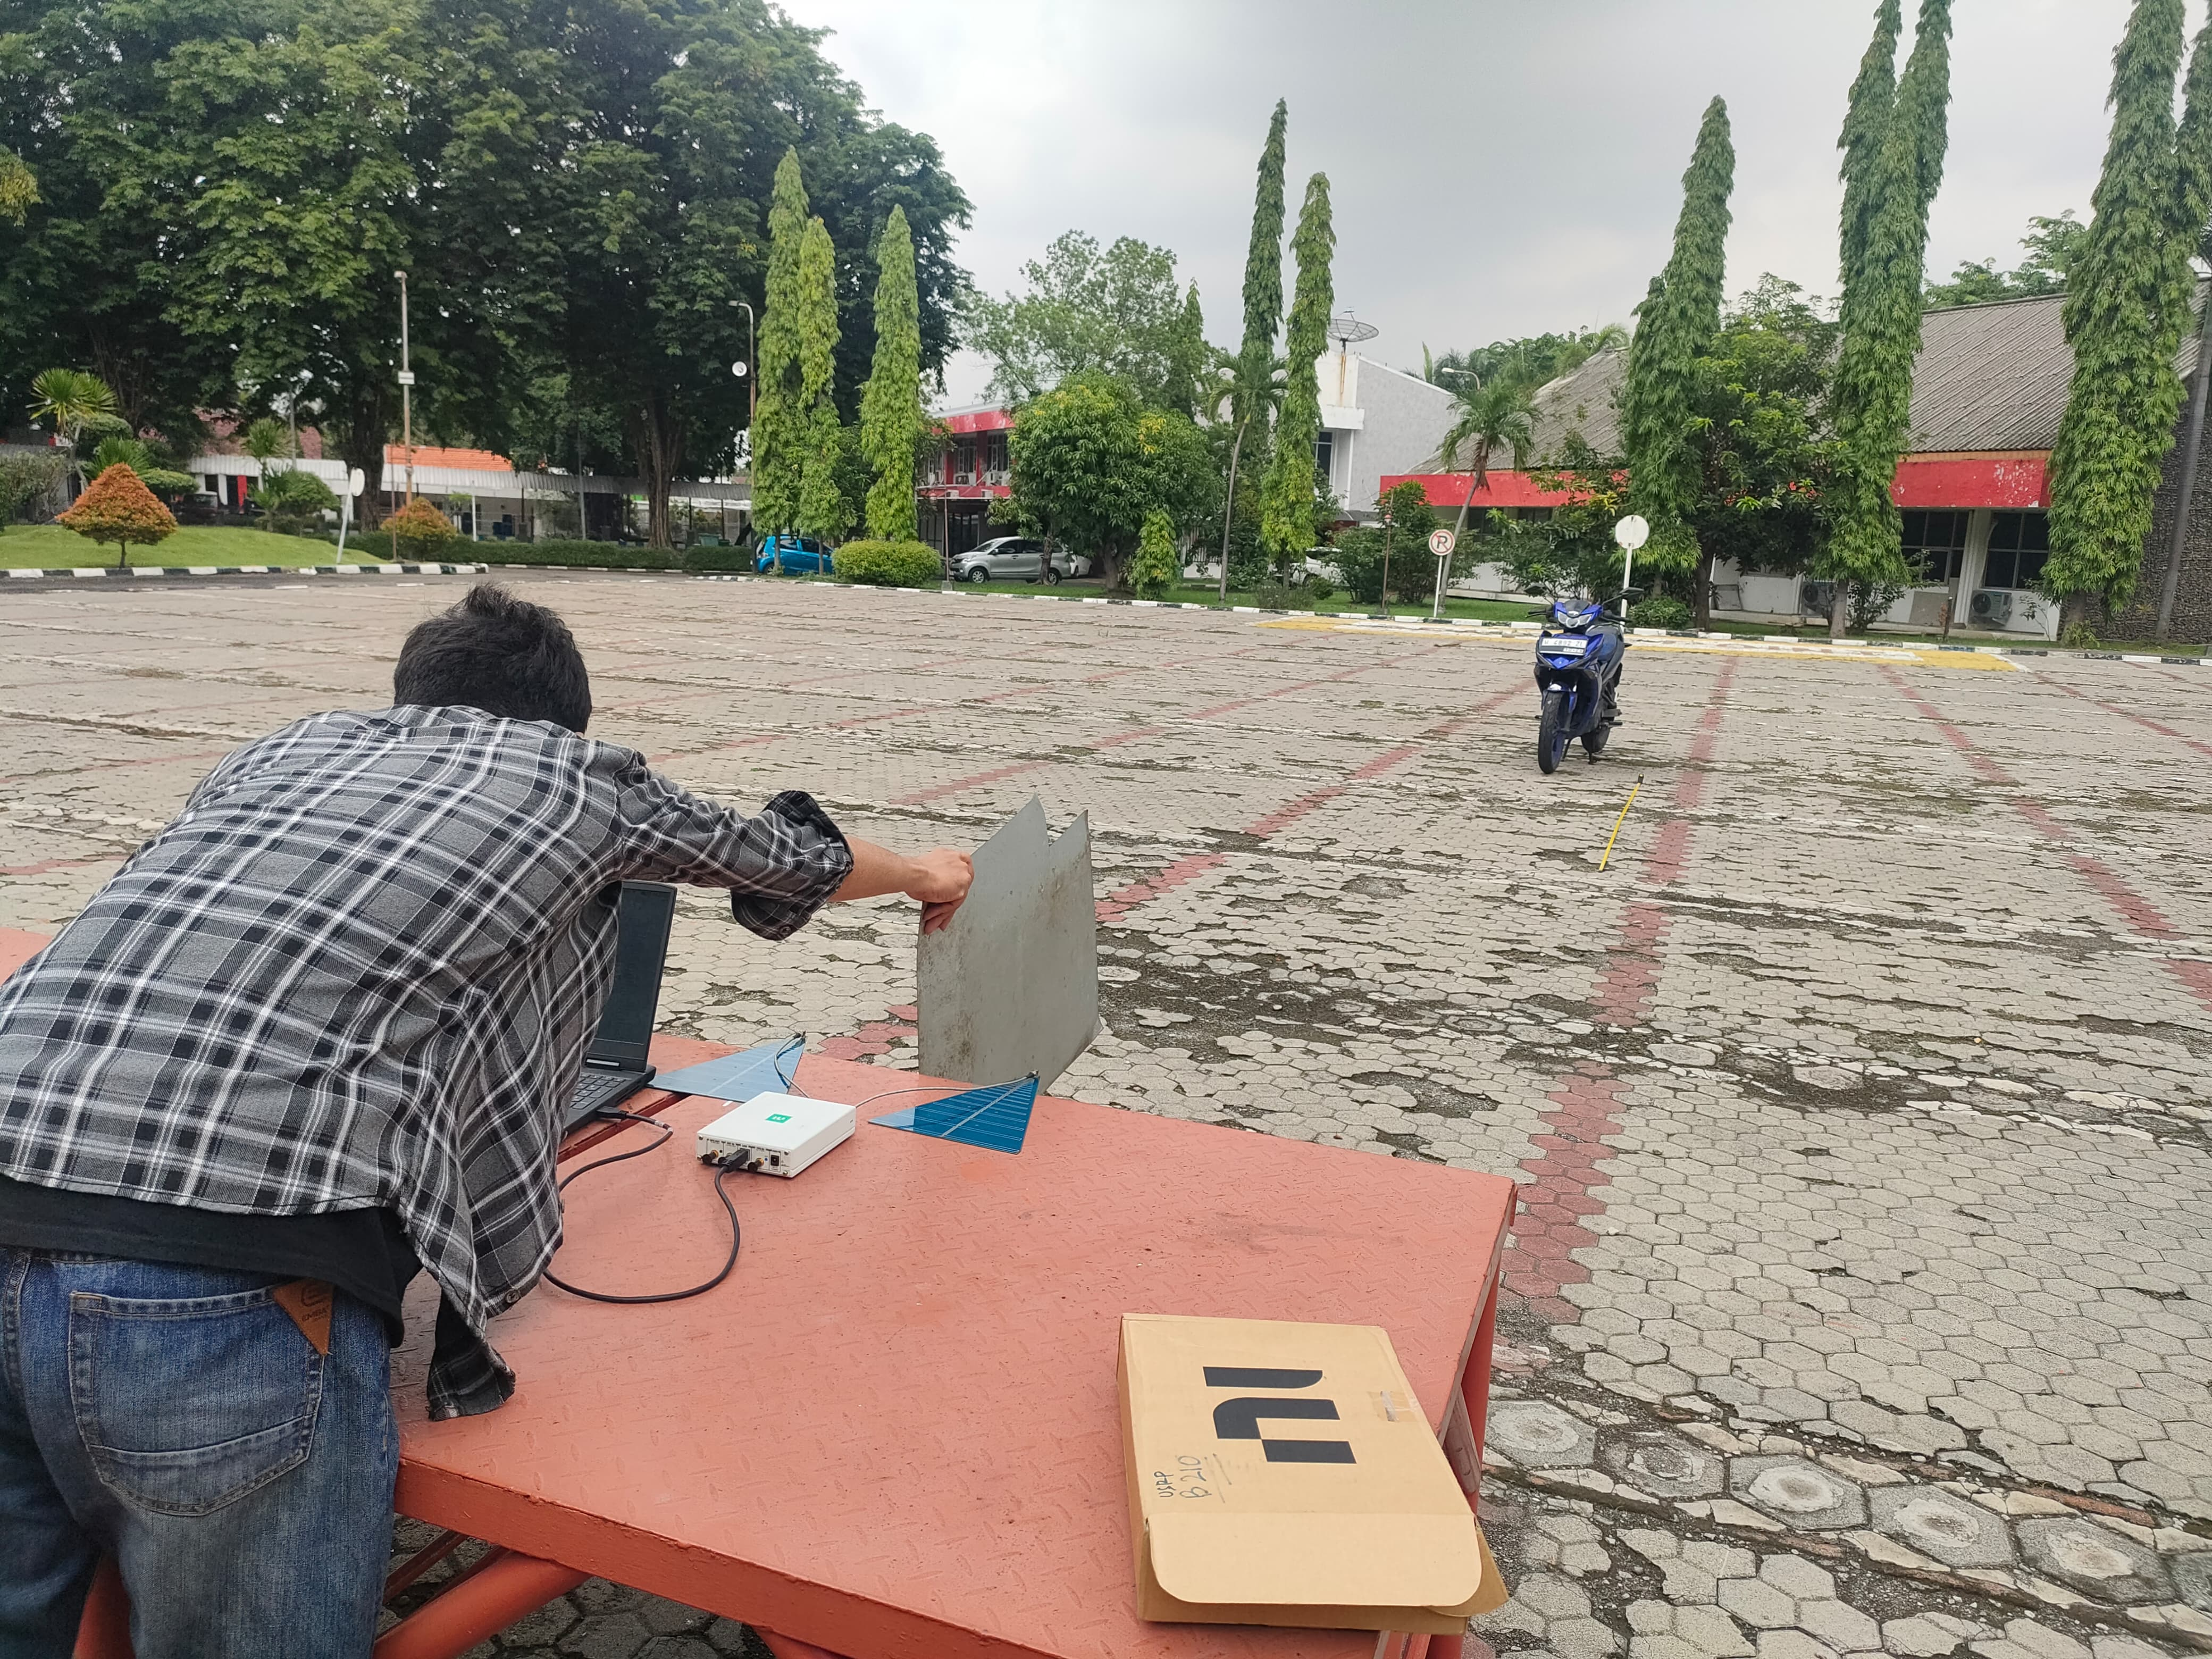
\includegraphics[scale=0.07]{pics/bab4/PengujianRange/9/Masuk.jpg}
	\caption{Pengambilan data jarak 9 meter}
	\label{fig:pengambilan9Meter}
\end{figure}
%-----------------------------------------------------------------------------%
\section{Pengambilan Data Kecepatan}
%-----------------------------------------------------------------------------%

Pengambilan data kecepatan dari objek dilakukan di tempat yang berbeda dengan pengambilan data jarak. Hal ini dikarenakan lintasan yang ada di lokasi pengambilan jarak tidak mendukung kecepatan hingga 20 km/h. Sehingga diputuskan bahwa pengambilan data kecepatan harus dilakukan ditempat lain yang memiliki lintasan mulus dan tidak membahayakan. Berbeda dengan pengambilan data jarak, pada data kecepatan diambil 2 skema yaitu mendekati radar dan menjauhi radar dengan 4 variasi kecepatan, masing masing kecepatan yang diuji dilakukan pengulangan sebanyak 3 kali. 

\subsection{Menjauhi Radar}

Pengambilan data menjauhi radar dilakukan dengan mengendarai kendaraan roda dua dekat dengan antena radar lalu melaju dengan kecepatan yang sudah ditentukan seperti pada gambar~\ref{fig:pengambilanMenjauhi}. Data akan terus diambil hingga 10 detik telah berlalu. Pembatasan pengambilan data ini dilakukan karena semakin lama data diambil, maka semakin besar pula data yang dihasilkan, sehingga pengolahan akan semakin berat untuk dilakukan.

\begin{figure}
	\centering
	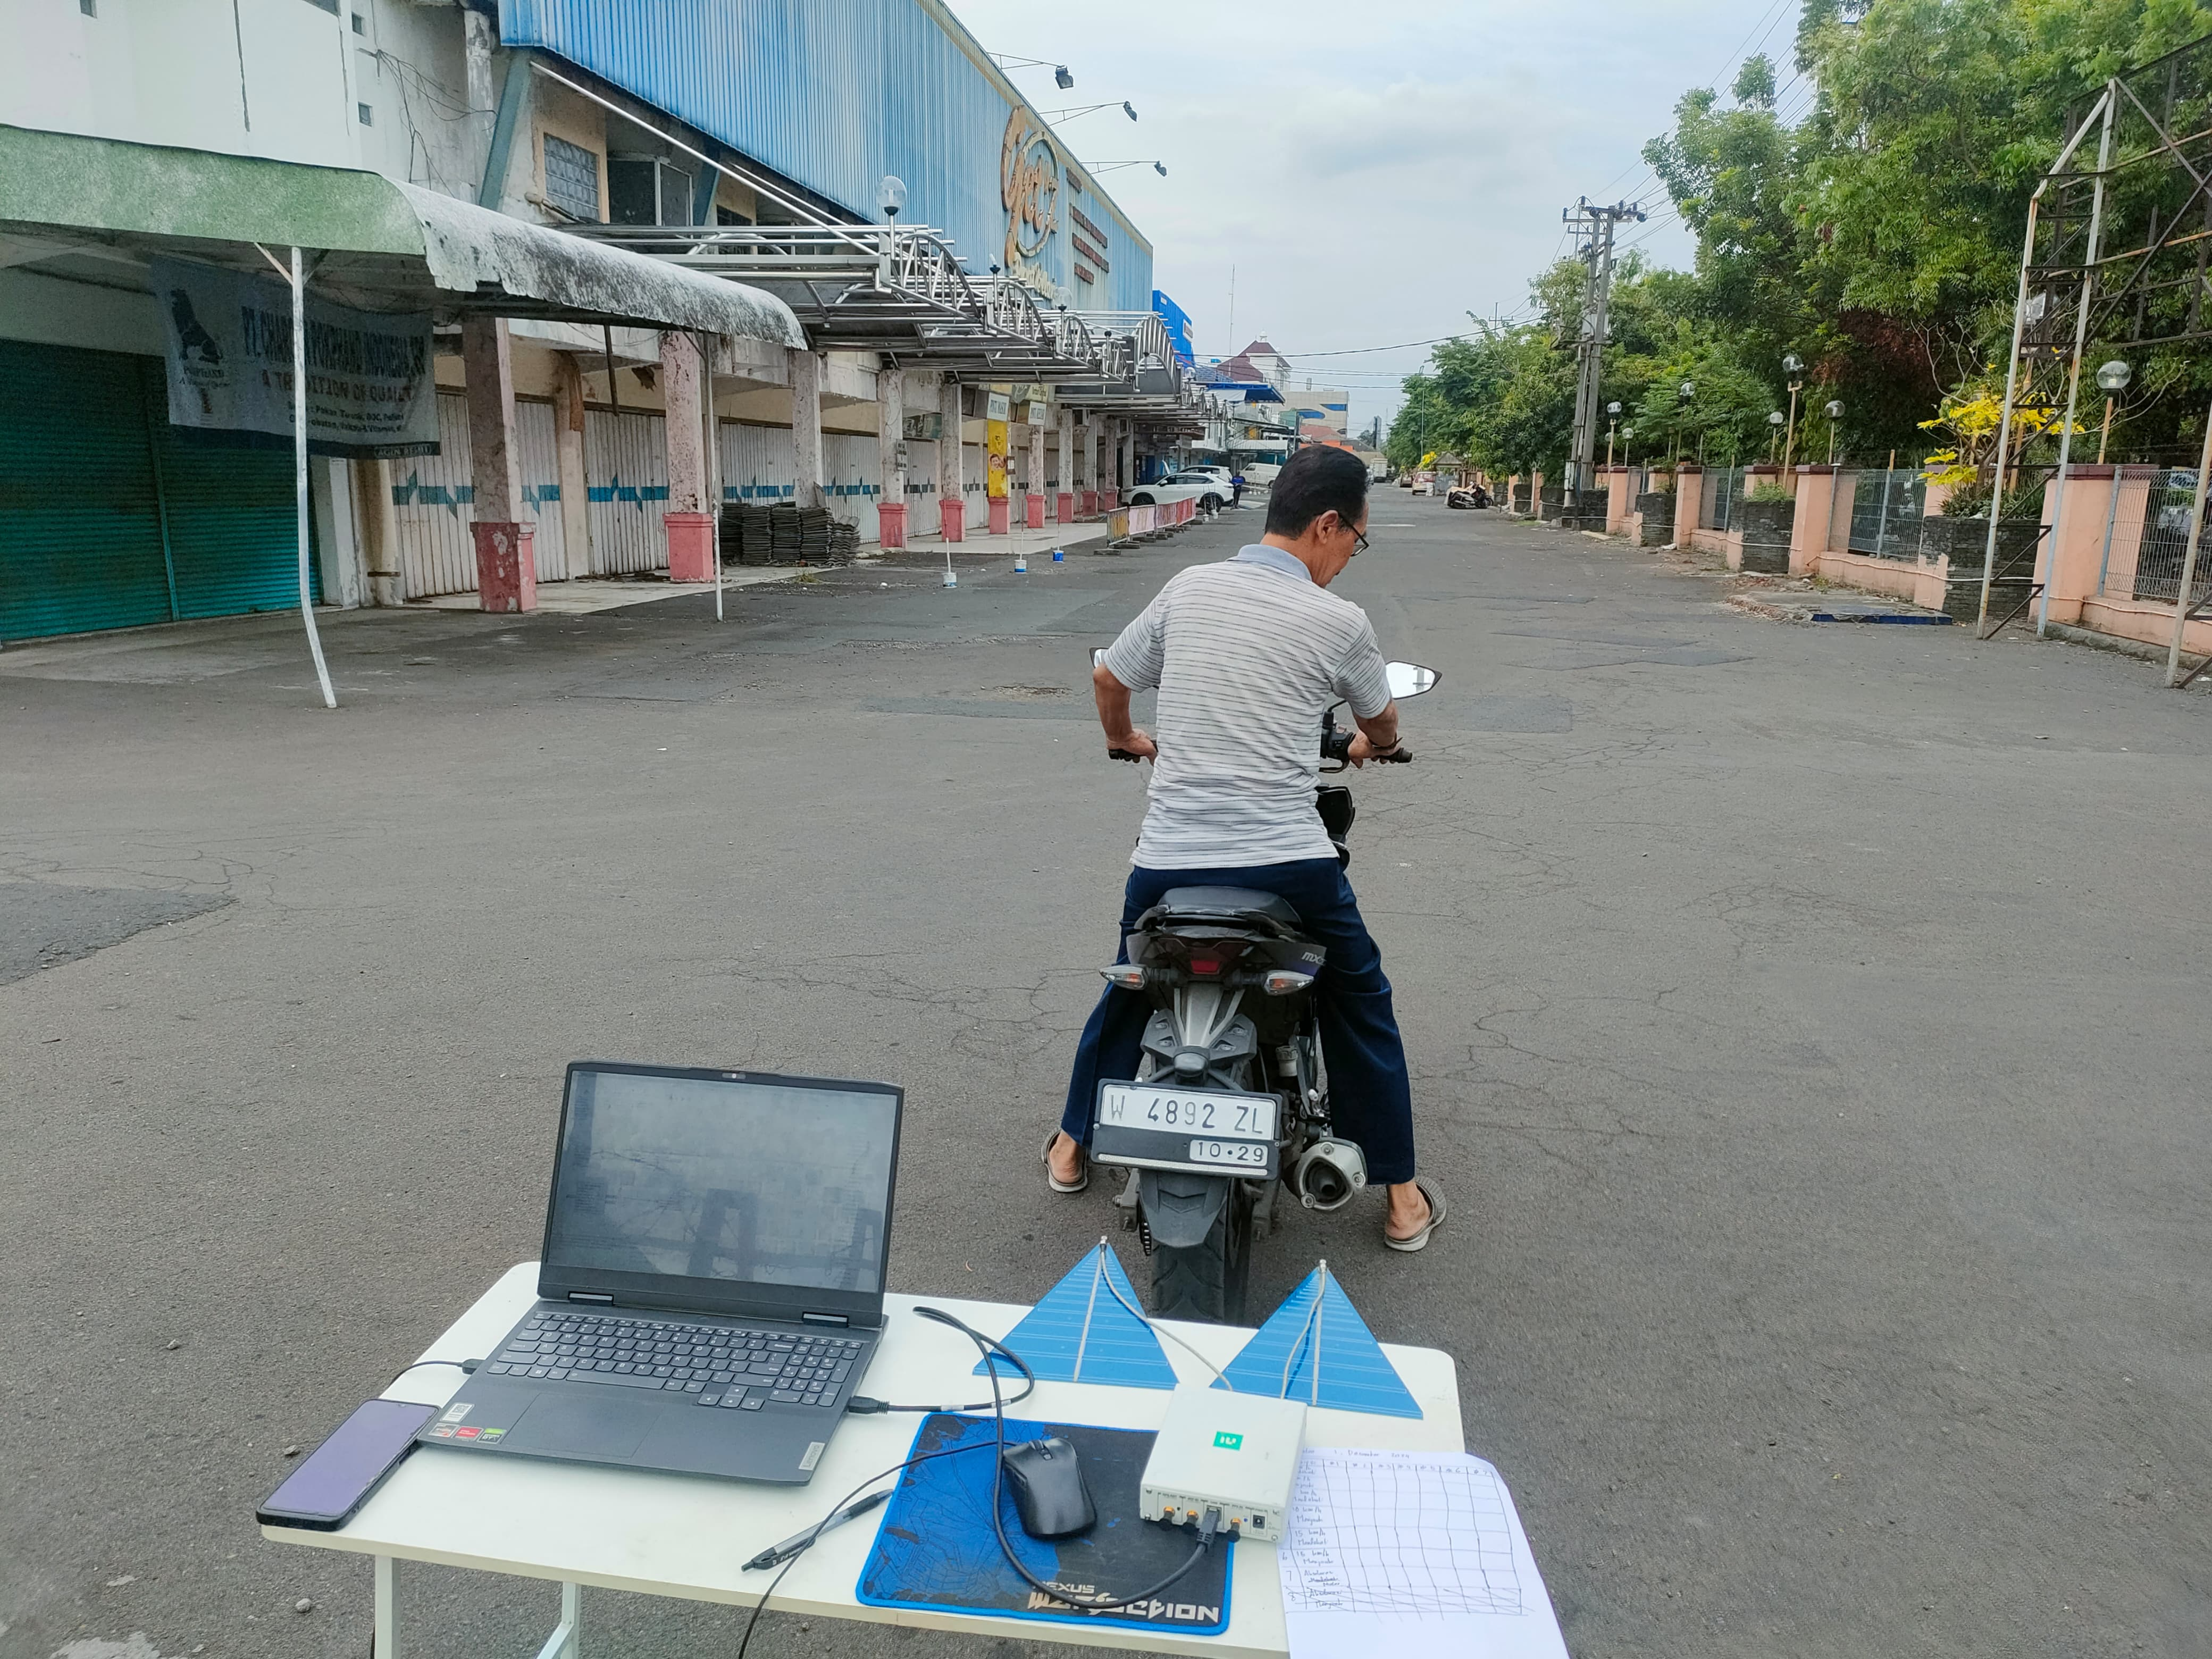
\includegraphics[scale=0.07]{pics/bab4/PengujianVelocity/1.jpg}
	\caption{Pengambilan data kecepatan menjauhi radar}
	\label{fig:pengambilanMenjauhi}
\end{figure}

\subsection{Mendekati Radar}

Pengambilan data mendekati radar dilakukan hampir sama dengan skema menjauhi radar, hanya saja jarak awal kendaraan ada pada sekitar 20 meter dari antena radar. Namun pemilihan jarak awal ini berubah, tiap kecepatan yang dipilih, pada pengukuran kecepatan lebih lambat, jarak awal yang dipilih lebih dekat dibanding kecepatan lebih tinggi. Hal ini dilakukan untuk memastikan kecepatan dari kendaraan bisa stabil di angka yang telah ditentukan. Gambar~\ref{fig:pengambilanMendekati} menunjukkan kegiatan pengambilan data yang telah dilaksanakan.

\begin{figure}
	\centering
	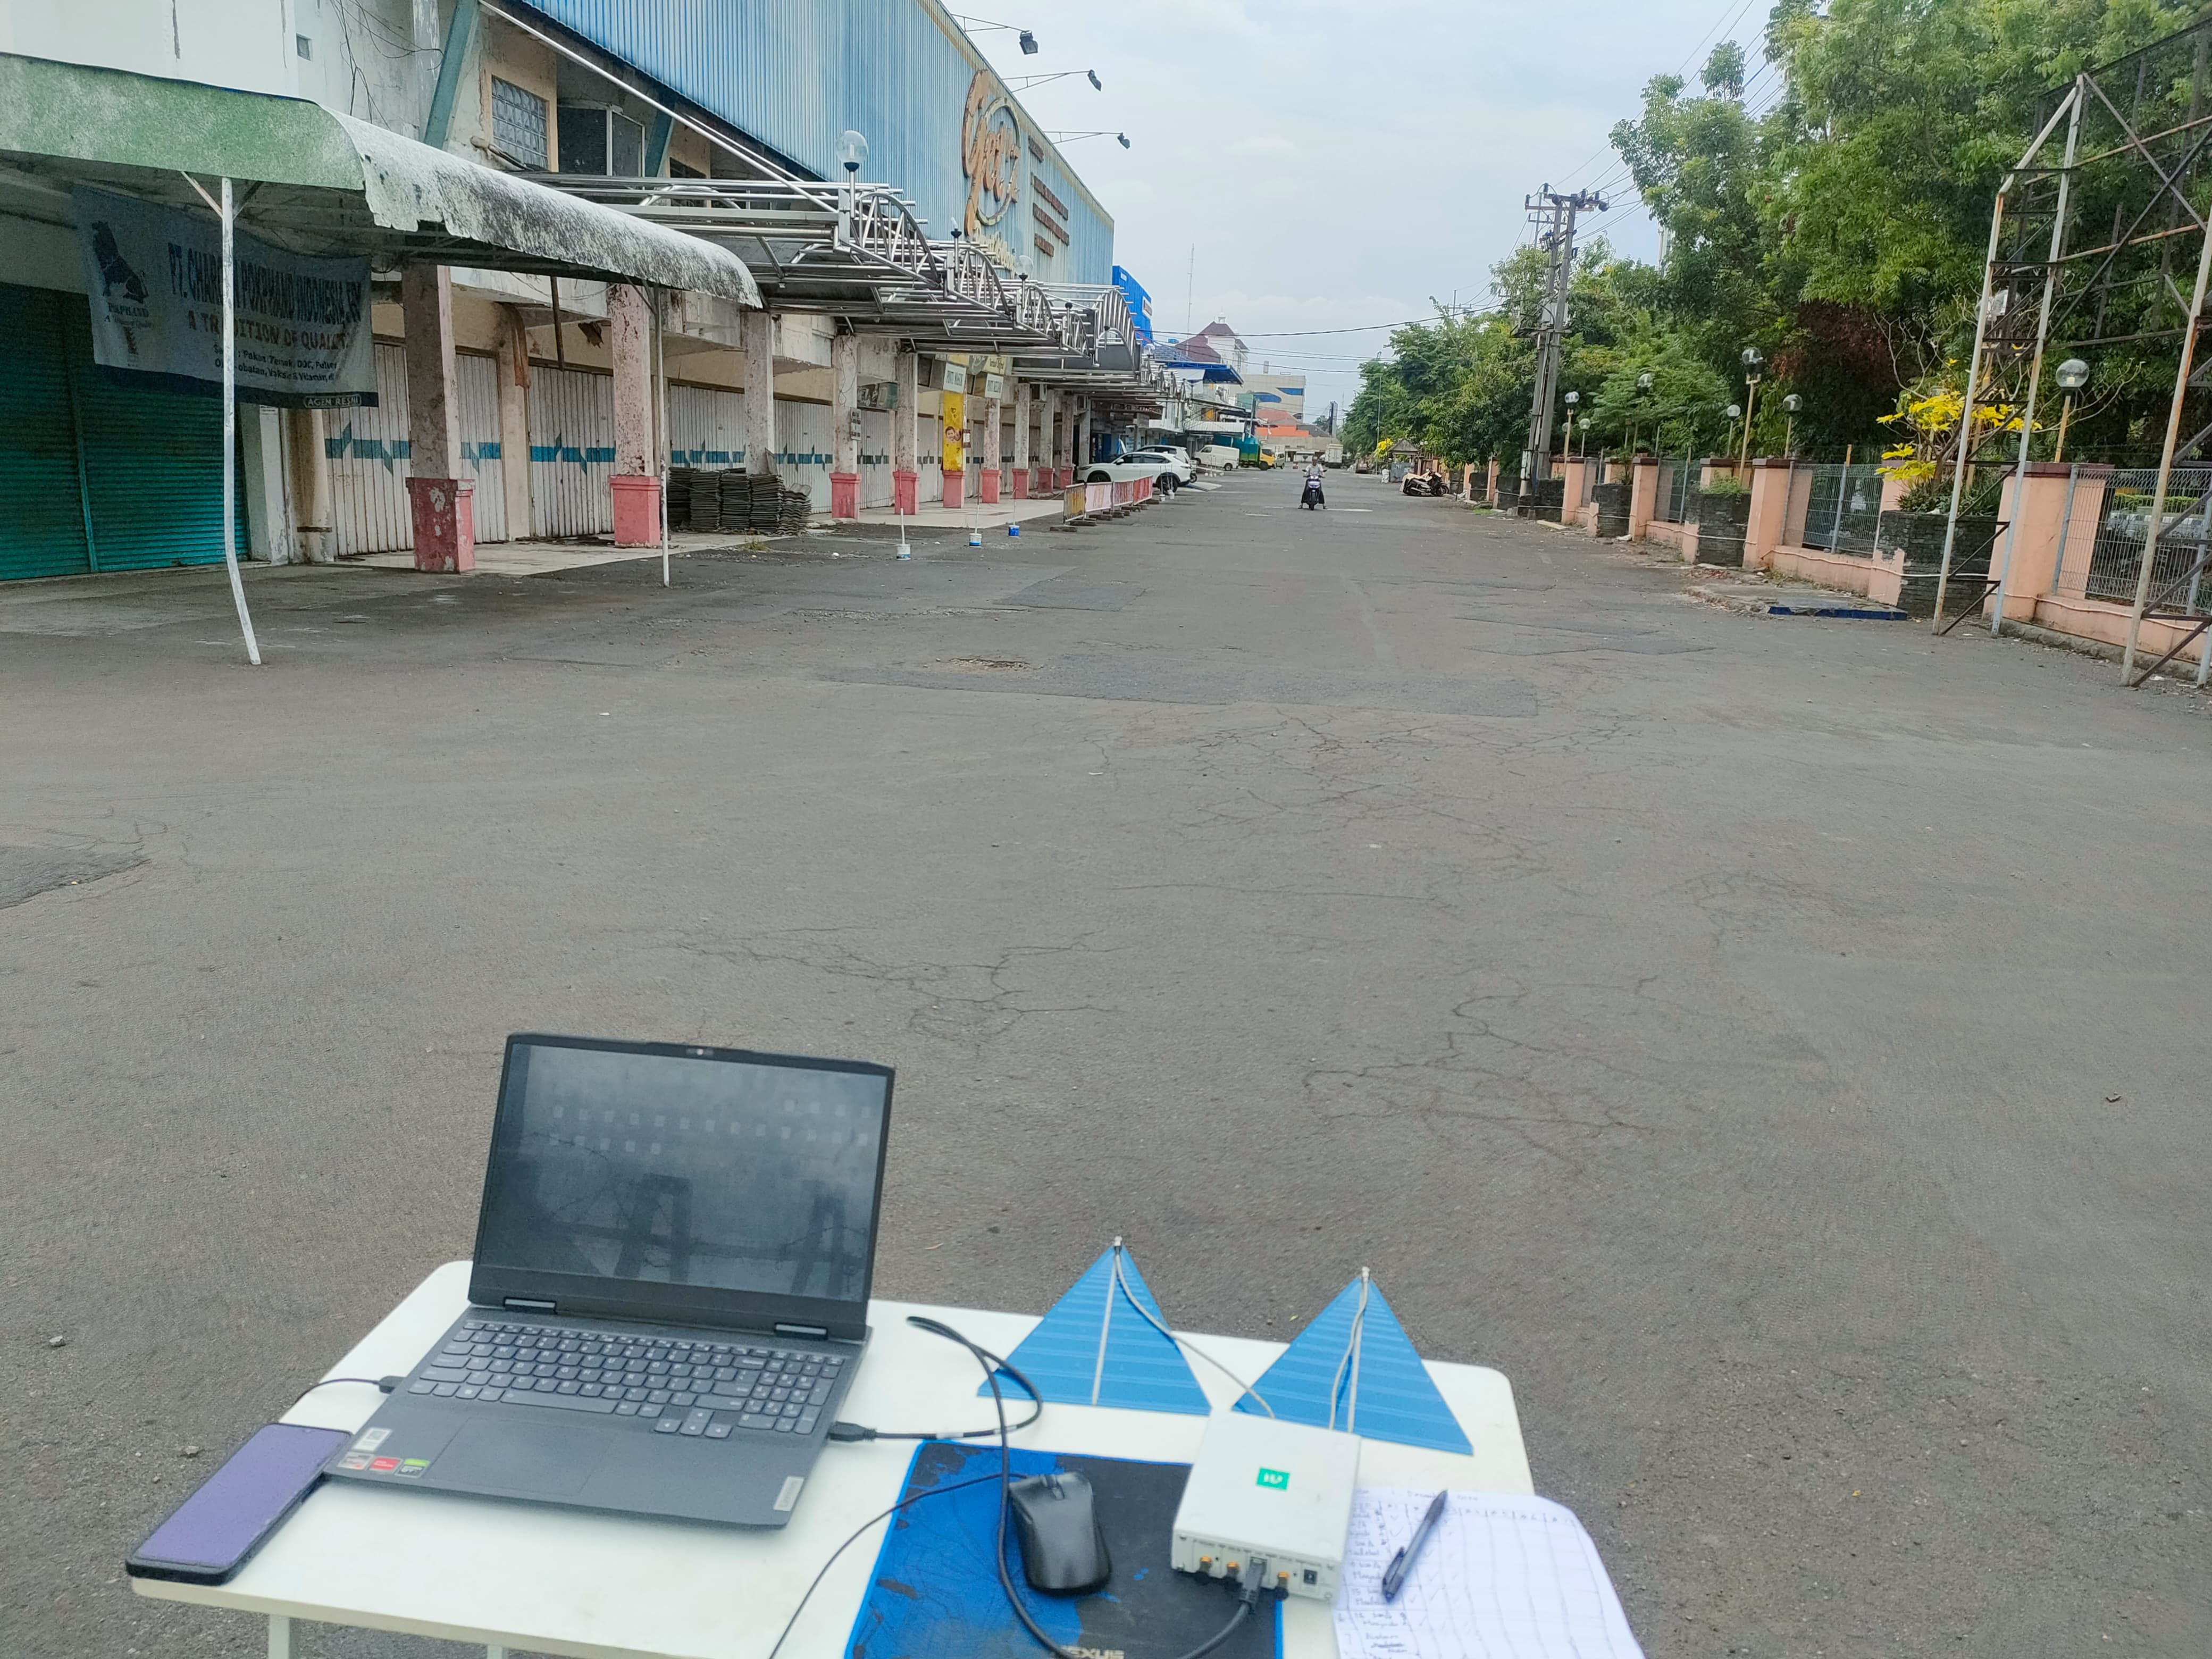
\includegraphics[scale=0.07]{pics/bab4/PengujianVelocity/3.jpg}
	\caption{Pengambilan data kecepatan mendekati radar}
	\label{fig:pengambilanMendekati}
\end{figure}

%-----------------------------------------------------------------------------%
\section{Pengolahan Data Dengan Matlab}
%-----------------------------------------------------------------------------%

Setelah dilaksanakan pengambilan data jarak objek dan kecepatan objek, selanjutnya adalah melakukan pengolahan dengan perangkat lunak matlab.

\subsection{Pengolahan Data Jarak}

Data jarak yang sudah didapat akan diolah dengan perangkat lunak matlab. Dengan melakukan perkalian \textit{conjugate} antara sinyal terkirim dan sinyal yang diterima, maka \textit{beat frequency} akan didapat. Saat nilai \textit{beat frequency} didapat, maka selanjutnya nilai tersebut bisa dimasukkan kedalam persamaan~\ref{eq:RangeEst}. Persamaan ini telah tersedia dalam bentuk fungsi di dalam perangkat lunak matlab, dengan memanggil \textit{beat2range(fb,slope)} dimana fb adalah nilai \textit{beat frequency} yang didapat dari pengolahan sebelumnya dan \textit{slope} adalah lebar \textit{sweep bandwidth} yang telah dipilih, yaitu 14 MHz. 

\subsection{Pengolahan Data Kecepatan}

Data kecepatan secara teori dilakukan dengan mengukur berapa pergeseran frekuensi yang terjadi antara frekuensi terkirim dan frekuensi yang diterima. Namun pada kenyataannya, data yang didapat memiliki \textit{phase noise}, seperti yang ditunjukkan pada gambar~\ref{fig:phaseNoise}. 

\begin{figure}
	\centering
	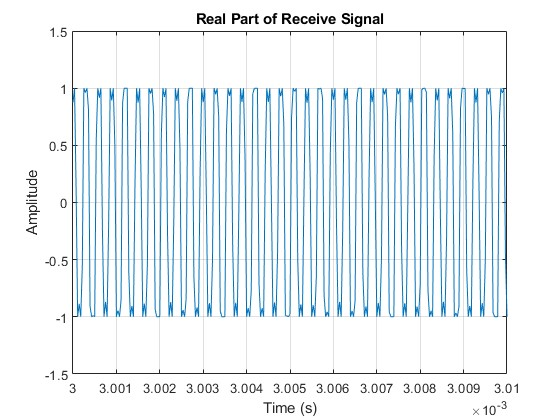
\includegraphics[scale=0.5]{pics/bab4/RealPartRx.jpg}
	\caption{\textit{Phase Noise} dari sinyal yang diterima}
	\label{fig:phaseNoise}
\end{figure}

Gambar~\ref{fig:phaseNoise} menunjukkan bagian real dari sinyal FMCW yang terpantul dari objek. Dapat dilihat pada fasa 90, selalu terjadi kerusakan sinyal, perlu diingat bahwa pengamatan sinyal ini dilakukan dalam waktu 0.01 detik. Saat seluruh sinyal diterima di plot dalam bentuk perubahan frekuensi dalam waktu, hal ini akan terlihat dengan jelas seperti dalam gambar~\ref{fig:instFreq}.

\begin{figure}
	\centering
	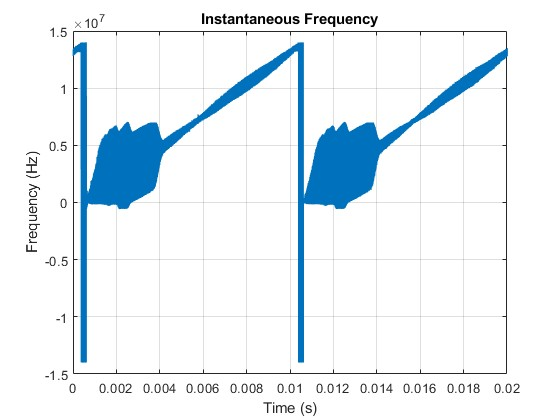
\includegraphics[scale=0.5]{pics/bab4/InstFreq.jpg}
	\caption{Perubahan frekuensi dengan waktu}
	\label{fig:instFreq}
\end{figure}

Nampak pada gambar~\ref{fig:instFreq} bahwa selalu ada \textit{phase noise} yang terjadi, sehingga saat sinyal yang di transmisi dan sinyal yang diterima dibandingkan, pengukuran kecepatan akan sangat sulit dilaksanakan, apalagi saat sinyal doppler yang terjadi sangat kecil. Sehingga digunakanlah teknik lain dalam mengukur kecepatan. Kecepatan dapat didefinisikan menggunakan persamaan sederhana kecepatan bersimbol V, dengan S dibagi t. S adalah jarak tempuh objek dan t adalah waktu tempuh objek. Dengan melakukan konversi dari minimal dua \textit{beat frequency} ke dalam jarak, dan melakukan kalkulasi terhadap perubahan waktu tersebut, maka nilai kecepatan akan didapat.

%\begin{equation}
%	V = \frac{S}{t}
%\end{equation}

 


%%--------------------------------%
%\todo{
	%\section{Simulasi Sistem}
	%Masukkan gambar simulasi pada gnuradio\\ 
	%Masukkan gambar hasil yang dilakukan dengan simulasi (berupa time vs frequency).\\
	%Masukkan proses analisis yang dilakukan dengan hasil simulasi, seperti langkah konversi biner ke kompleks, penentuan data yang diambil,... pada matlab.\\
	%Lakukan desain blok dari hasil pada matlab menuju python.\\
	%Uji coba blok python yang telah dirancang pada simulasi\\
	%Bandingkan hasilnya dengan pada matlab
	%}
%%--------------------------------%
